\section{模型评价}
\subsection{模型评价}
\subsubsection{模型优点}
\begin{enumerate}
\item 运用蒙特卡洛方法计算阴影遮挡效率和截断效率,避免求解
\item 
\end{enumerate}

\subsubsection{模型缺点}
\begin{enumerate}
\item 计算阴影遮挡效率的算法运行效率低,仍有改进优化的空间。
\item 在问题2之中设计镜场布局时,为了简化模型,只考虑了上文所描述的均匀布局,该布局效率较低,而在实际的镜场设计过程之中,可以叶序螺线(phyllotaxis spiral)布局,又称仿生布局(biomimetic layout)以及阿基米德螺线(Archimedean spiral)布局等\cite{noone},如下图所示:
\begin{figure}[H]
\centering
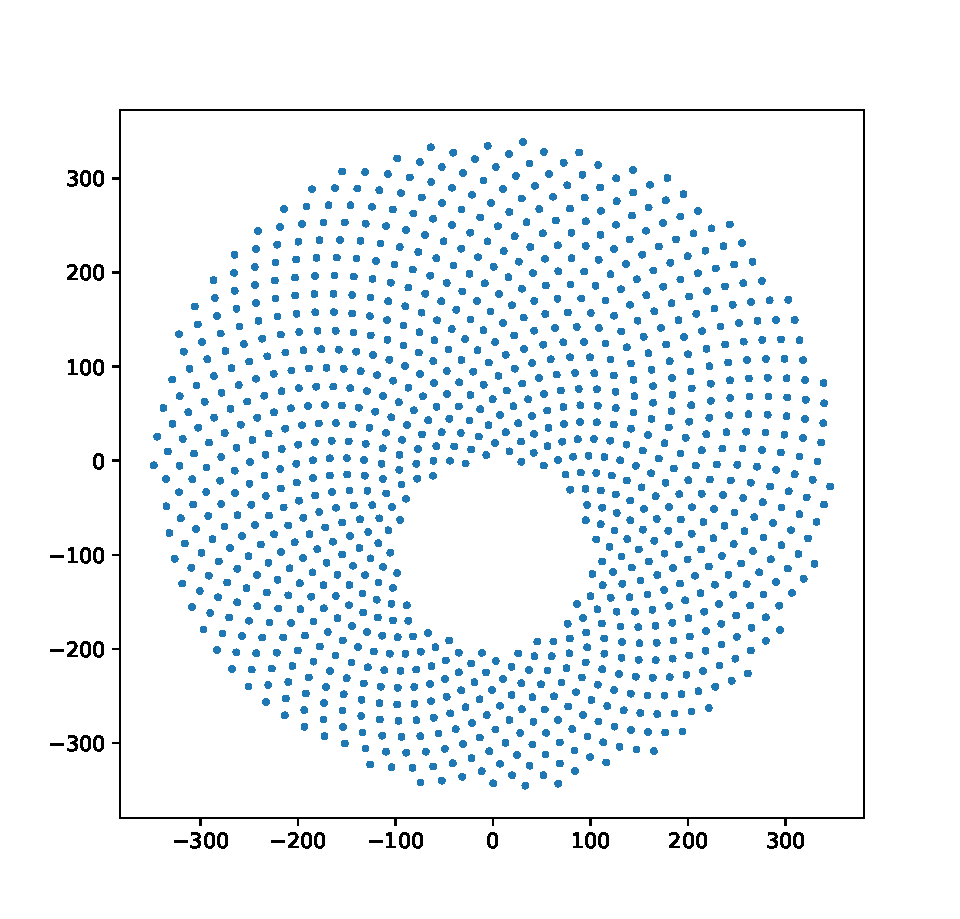
\includegraphics[scale = 0.5]{yexu.pdf}
\caption{\kaishu 叶序螺线}
\end{figure}
\end{enumerate}
